\documentclass[11pt,openright,twoside]{report}
\usepackage[utf8]{inputenc}
\usepackage[hmargin=4cm,vmargin=3.5cm,bmargin=3.5cm]{geometry}
\usepackage[portuguese, english]{babel}
\usepackage{graphicx}
\usepackage{hyperref}
\usepackage{indentfirst}
\usepackage{listings}
\usepackage{color}
\usepackage{float}

\definecolor{dkgreen}{rgb}{0,0.6,0}
\definecolor{gray}{rgb}{0.5,0.5,0.5}
\definecolor{mauve}{rgb}{0.58,0,0.82}

\lstnewenvironment{Java}{
	\lstset{frame=tb,
  	language=Java,
  	aboveskip=3mm,
  	belowskip=3mm,
  	showstringspaces=false,
  	columns=flexible,
  	basicstyle={\small\ttfamily},
  	numbers=none,
  	numberstyle=\tiny\color{gray},
  	keywordstyle=\color{blue},
  	commentstyle=\color{dkgreen},
  	stringstyle=\color{mauve},
  	breaklines=true,
  	breakatwhitespace=true,
  	tabsize=3,
  	comment=[l]{//},
	}
}{}

\lstnewenvironment{Python}{
	\lstset{frame=tb,
  	language=python,
  	aboveskip=3mm,
  	belowskip=3mm,
  	showstringspaces=false,
  	columns=flexible,
  	basicstyle={\small\ttfamily},
  	numbers=none,
  	numberstyle=\tiny\color{gray},
  	keywordstyle=\color{blue},
  	commentstyle=\color{dkgreen},
  	stringstyle=\color{mauve},
  	breaklines=true,
  	breakatwhitespace=true,
  	tabsize=3,
  	comment=[l]{\#},
	}
}{}

\renewcommand{\rmdefault}{phv}
\renewcommand{\sfdefault}{phv}
\renewcommand{\baselinestretch}{1.1}


\title{\textbf{Relatório - Python vs Java}}

\begin{document}

\begin{titlepage}
\begin{figure}
\title{\textbf{Relatório - Python vs Java}}
\author{Turma 2 - Diogo Ferreira e Luís Leira\\\vspace{3cm}
Universidade de Aveiro - Laboratórios de Informática}
\date{\today}
 
\includegraphics[scale=1.5]{ua_logo.png}
\end{figure}
\end{titlepage}

\selectlanguage{portuguese}
\maketitle
\tableofcontents
\listoffigures

\part{Apresentação}

\chapter{Resumo}
Neste trabalho são apresentadas comparações entre as linguagens Python e Java. Começando pela sua apresentação, expomos a história, o objetivo e onde é usada cada linguagem, tentando não transparecer para já qualquer detalhe semântico. Após este capítulo inicial, começamos por comparar semanticamente e lexicalmente as linguagens, percorrendo os seus elementos básicos, tipos de dados e variáveis, operadores, leitura e escrita de dados, estruturas de decisão e de controlo, classes, funções, arrays/listas/dicionários e ficheiros. Na última parte deste capítulo, iremos comparar aspetos funcionais das linguagens como a portabilidade, a velocidade de execução, a facilidade de uso e estatísticas globais. Por fim, fazemos uma conclusão onde nos iremos concentrar nas vantagens de uma linguagem em relação à outra e para que fins se podem destinar.

\chapter{Introdução}
Neste relatório iremos explorar duas linguagens de programação (Java e Python, \autoref{pythonvsjava}) comparando-as entre si. Atualmente, há muitas dúvidas sobre por que linguagem se deve começar por aprender, e sobre quais são as vantagens de uma sobre a outra. Como são duas das linguagens mais usadas mundialmente, há opiniões divididas sobre o caso.
No entanto, não há como negar que são linguagens usadas para propósitos diferentes e com princípios diferentes. Iremos expor essas diferenças tal como também aquilo em que se assemelham, e iremos também fundamentar qual linguagem poderá ser mais conveniente usar consoante o que é pretendido.

\begin{figure}[H]
 \center
 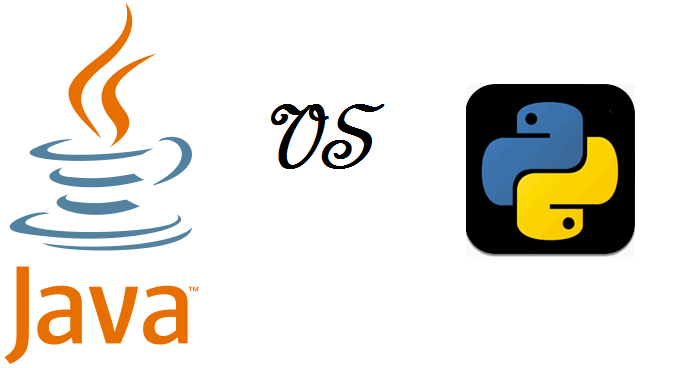
\includegraphics[scale=.5]{pythonvsjava.png}
 \caption{Símbolos do Java (à esquerda) e do Python (à direita). Fonte: http://commons.wikimedia.org/ (montagem realizada por Diogo Ferreira).}
 \label{pythonvsjava}
\end{figure}

\part{Desenvolvimento}

\chapter{Apresentação das linguagens}
\subsubsection{Python}
Python surgiu em 1991 e foi criada por Guido van Rossum. Sucessora da linguagem \textit{ABC}, tem como objetivo enfatizar a produtividade do programador sobre a velocidade de execução. É uma linguagem de alto nível, interpretada, orientada a objetos e de tipagem dinâmica (conceito que será explicado no próximo capítulo). Sendo interpretada, não é compilada, apenas executada diretamente do seu código-fonte. Possui um modelo de desenvolvimento comunitário aberto. A sua filosofia centra-se na facilidade de leitura de código e rapidez de desenvolvimento, quando comparado com C++ ou Java. O nome escolhido foi Python, não devido ao réptil (pitão), mas em homenagem ao famoso grupo de comédia \textit{Monty Python's Flying Circus}. No comando "import this", implementado como um \textit{Easter Egg}, é possível ver \textit{The Zen Of Python}, descrevendo sumariamente a filosofia de Python (\autoref{zenofpython}).

\begin{figure}
 \center
 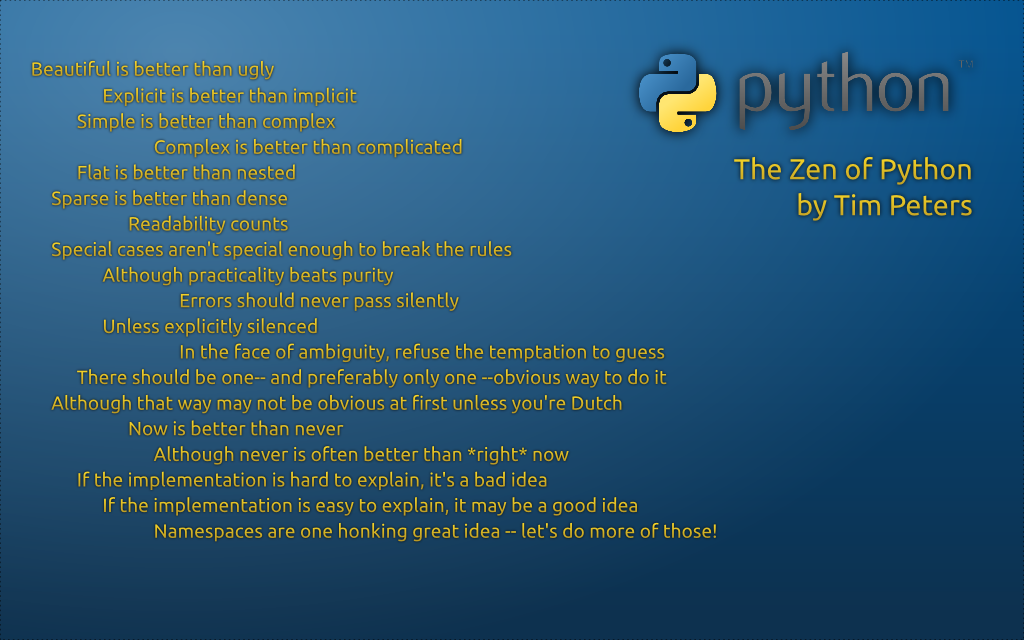
\includegraphics[scale=.4]{1024}
 \caption{\textit{The Zen of Python}, escrita por Tim Peters. Fonte: http://studley13.deviantart.com/}
 \label{zenofpython}
\end{figure}

Hoje em dia, Python está na versão 3.x e é utilizado com variados fins como linguagem de scripting. Pode ser utilizado, por exemplo, para aplicações web (i.e. Apache Web Server), servidores e interação entre API's (i.e. Dropbox, BitTorrent, Mercurial). Também pode ser utilizado em software mais complexo, como jogos (Civilization IV, Frets On Fire, World of Tanks, Battlefield 2), aplicações científicas ou aplicações de edição de vídeo e imagem (Cinema 4D, Lightwave, GIMP, Blender). Por último, algumas distribuições Linux utilizam Python como o instalador por defeito no terminal (Ubuntu usa Ubiquity, Red Hat e Fedora usam Anaconda, Gentoo usa Portage) (\cite{Python}).
\medskip

\subsubsection{Java}
Java é uma linguagem de programação criada em 1995 por um grupo de investigadores da Sun Microsystems, de onde se destaca James Gosling como seu principal criador. Foi originalmente desenhada para televisão interativa com o nome \textit{Oak}, mas nunca foi realmente usada com esse propósito (\cite{Java}). É uma linguagem concorrente, orientada a objetos e portável. O código Java é executado apenas sobre uma máquina virtual de Java, assegurando assim a compatibilidade entre sistemas. Em 2006 e 2007, todo o código-fonte da linguagem foi disponibilizado como open-source pela Sun Microsystems. Alguns dos princípios fundamentais da linguagem são:
\begin{itemize}
  \item Tem de ser simples, orientada a objetos e familiar
  \item Tem de ser robusta e segura
  \item Tem de ser compatível com diferentes sistemas
  \item Tem de ser interpretada e dinâmica
  \item Tem de ter uma boa \textit{performance}
\end{itemize}
Com a primeira versão lançada em 1996, a linguagem já vai na sua oitava versão (Março de 2014) e é atualmente uma das linguagens de programação mais usadas mundialmente. Tem três usos principais: uso no desktop, no Java Runtime Environment (em aplicações como MATLAB, NetBeans, LimeWire ou Vuze); uso mobile, principalmente por meio de software Android e suas aplicações; uso comercial e Web Server, como aplicações \textit{client-server} (Spring Framework, Hibernate, Apache TomCat) (\cite{Java}).

\chapter{Comparações entre as linguagens}

\subsection{Elementos básicos das linguagens}

\subsubsection{Exemplo de um programa básico}
\smallskip
\begin{Python}
# encoding=utf-8

print "Hello World"
\end{Python}
\smallskip

Este programa em Python apenas escreve no ecrã "Hello World", através da função \textit{print}. O encoding no topo é um indicador para o código ser lido como codificado em \textit{utf-8}.

\smallskip
\begin{Java}
public class Demo{
	public static void main(String[] args){
		System.out.print("Hello World");
	}
}
\end{Java}
\smallskip

Este programa em Java irá fazer exatamente o mesmo que o programa anterior. Primeiro, criamos a classe \textit{Demo}, que tem que coincidir com o nome do ficheiro para o compilador poder ler. A seguir, abrimos a função main, onde se encontra todo o nosso programa. Por fim, chamamos a função \textit{print} para escrever "Hello World" no ecrã.
\medskip

\subsubsection{Palavras reservadas}
Cada linguagem tem as suas palavras reservadas, isto é, palavras que não podem ser declaradas como variáveis porque implicam alguma coisa no contexto da linguagem. Como ambas as linguagens são \textit{case-sensitive}, as letras maiúsculas são diferentes das minúsculas para a interpretação de código, o que implica, por exemplo, que "and" não é o mesmo que "And" (embora não seja recomendável usar variáveis iguais apenas com diferenças nas maiúsculas!).
\smallskip

Em Python 2.x, existem 31 palavras reservadas:

\begin{table}[h]
\begin{tabular}{lllllll}
and					    & continue    	& except    & global    & lambda   & raise & yield\\
as                  	& def    	  	& exec 		& if 	& not    & return    \\
assert                  & del   		& finally     & import  & or  & try  \\
break                   & else   		& for    	& in     	& pass & while  \\
class                	& elif 			& from  	& is 		& print & with
\end{tabular}
\end{table}
\smallskip

Já em Java, existem 52 palavras reservadas:

\begin{table}[H]
\begin{tabular}{lllll}
abstract & continue & for        & new       & switch       \\
assert   & default  & goto       & package   & synchronized \\
boolean  & do       & if         & private   & this         \\
break    & double   & implements & protected & throw        \\
byte     & else     & import     & public    & throws       \\
case     & enum     & instanceof & return    & transient    \\
catch    & extends  & int        & short     & try          \\
char     & final    & interface  & static    & void         \\
class    & finally  & long       & strictfp  & volatile     \\
const    & float    & native     & super     &             
\end{tabular}
\end{table}
\medskip

\subsubsection{Indentação}
A maioria das linguagens ignora os espaços em branco e os parágrafos criados quando é compilada. É assim com Java, que divide os seus módulos com chavetas.
\begin{Java}
public class Demo{								// Inicio de um bloco maior (Demo)
	public void main (String[] args){			// Inicio de outro bloco
		System.out.print("Aveiro");
	}											// Final de um bloco
}												// Final de outro bloco
\end{Java}
\smallskip

Normalmente, a estética indica que devemos sempre indentar o código de acordo com o bloco a que corresponde. No entanto, nada nos impede de escrevermos um programa inteiro na mesma linha (não recomendável!).
\smallskip

Em Python, os blocos não se explicitam por chavetas, mas por indentação. Ou seja, se não indentarmos o código corretamente (um parágrafo com quatro espaços antes de um novo bloco), ele dará erro.

\begin{Python}
# encoding=utf-8

a=2
i=0
while i!=a:		# O que esta intrucao faz iremos explicar a frente.
	print i 		# Quatro espacos (1 paragrafo) de distancia do inicio, para #indicar o interior de um bloco
	i+=1
\end{Python}
\medskip

\subsubsection{Comentários}
Os comentários são notas que podem ser introduzidas com o intuito de melhorar a legibilidade do código. Os mesmos são ignorados quando o programa é executado, não introduzindo quaisquer modificações no programa.
\smallskip

Em Python é introduzido um comentário através do caracter '\#' que termina no final da linha.

\smallskip
\begin{Python}
# Um comentario pode servir para apresentar o que faz um bloco de
# codigo. Neste caso, podemos ver uma declaracao da variavel a
a = 2
\end{Python}
\smallskip

Em Java utiliza-se '//' quando se pretende que o comentário termine no final da linha. Para comentários de uma ou mais linhas também se pode utilizar '/*' para inicializar e '*/' para terminar.

\smallskip
\begin{Java}
//Declaracao de variaveis
int a = 4;
/* Desta forma podemos escrever
um comentario mais longo */
\end{Java}
\medskip

\subsection{Tipos de dados e variáveis, operadores, leitura e escrita de dados e estruturas de decisão e de controlo}

\subsubsection{Tipos de dados e variáveis}
\medskip

\textbf{Tipos de dados}
\smallskip

Em Python existem os seguintes tipos de dados mais comuns:

\begin{table}[h]
\begin{tabular}{|l|l|}
\hline
bool & Corresponde a um valor booleano, ou armazena "true", que representa "1", ou "false", \\
& representando "0".            \\
\hline
int     & Armazena 32 bits de informação de números inteiros.                               \\
\hline
long    & Armazena 64 bits de informação de números inteiros.                               \\
\hline
float   & Armazena 32 bits de informação representando um número decimal (real).            \\
\hline
complex   & Armazena um número complexo no formato A+Bi onde A corresponde à parte real     \\
& e B à parte imaginária.            \\
\hline
str    & Corresponde a uma String e armazena um conjunto de 8 caracteres.        \\
\hline
unicode   & Corresponde a uma String e armazena um conjunto de 32 caracteres unicode.                                                          \\             
\hline                                                                      
\end{tabular}
\end{table}

Ainda em Python, é relevante referir que não existe o tipo char (ao contrário do que acontece em Java, como veremos a seguir).

\smallskip

Em Java, antes de utilizar uma variável é preciso inicializá-la (demonstrado a seguir). Existem oito tipos possíveis de dados primários:
\begin{table}[h]
\begin{tabular}{|l|l|}
\hline
boolean & Ou armazena "true", que representa "1", ou "false", representando "0".            \\
\hline
byte    & Armazena apenas 8 bits de informação, ou seja, um número entre -128 e 127.        \\ \hline
short   & Armazena 16 bits de informação, ou seja, um número inteiro entre -32.768 e 32.767.\\
\hline
int     & Armazena 32 bits de informação de números inteiros.                               \\
\hline
long    & Armazena 64 bits de informação de números inteiros.                               \\
\hline
float   & Armazena 32 bits de informação representando um número decimal (real).            \\
\hline
double  & Armazena 64 bits de informação representando um número decimal (real).            \\
\hline
char    & Armazena um carácter.                                                           \\                                                                                
\hline
\end{tabular}
\end{table}

Também é possível inicializar uma String, que é um conjunto de caracteres, não sendo um tipo de dado primitivo de Java.
Em Python, não é necessário inicializar qualquer tipo de variável, pois são atribuídos de forma dinâmica.
\medskip

\textbf{Inicialização de variáveis}
\smallskip

Em Python, a inicialização de variáveis dá-se sem ser necessário declarar o tipo de variável. Isto implica que quando se dá a inicialização, o tipo da variável é introduzido quando é atribuído um valor. É uma linguagem de tipagem dinâmica, sendo possível atribuir um valor de outro tipo (que não o inicial), ao contrário do que acontece em Java. Este caso encontra-se exemplificado a seguir.

\smallskip
\begin{Python}
# encoding=utf-8

mes = 3 # Declaracao de uma variavel mes do tipo int atraves da #atribuicao do valor 2015
mes = "marco" # Atribuicao do valor marco a variavel mes, passando a ser #uma string
\end{Python}
\smallskip

Ao contrário do que acontece em Python, em Java é necessário identificar antecipadamente o tipo da variável que se quer inicializar (isto é, antes de lhe atribuir um valor), sendo portanto uma linguagem de tipagem estática. Uma variável não pode mudar o seu tipo, como referido anteriormente.

\smallskip
\begin{Java}
public class Demo{
	public void main (String[] args){
		int mes = 3; // Declaracao de uma variavel mes do tipo int e //atribuicao do valor 3
	}
}
\end{Java}
\smallskip

O facto das linguagens serem de tipagens diferentes, cada uma delas apresenta características específicas. As principais vantagens, em geral, de uma em relação à outra são as seguintes: a tipagem dinâmica (presente em Python) confere maior flexibilidade, maior rapidez no processo de desenvolvimento e maior concisão, enquanto que a tipagem estática (presente em Java) confere maior segurança, maior performance e maior legibilidade do código.
\medskip

\subsubsection{Operadores aritméticos, de comparação e lógicos}
Em ambas as linguagens, há operadores numéricos bastante semelhantes. Para a aritmética, ambas as linguagens possuem "+" (adição), "-" (subtração), "*" (multiplicação), "/" (divisão) e "\%" (módulo). Em Python, "**" significa elevar alguma coisa ao expoente, enquanto que "//" é uma divisão com arredondamento por defeito. Em Java, também há "++" (adicionar um valor a alguma variável, ou seja, incremento) ou "\---" (retirar um valor a alguma variável, ou seja, decremento).
\smallskip

Os operadores de comparação são iguais para as duas linguagens: "==" verifica se é igual, "!=" verifica se é diferente, " \textless " verifica se é menor, " \textgreater " verifica se é maior, " \textless =" verifica se é menor ou igual e " \textgreater =" verifica se é maior ou igual.
\smallskip

Para não tornar este tema demasiado extenso, apenas iremos falar de alguns operadores lógicos. Para Java, "\&\&" é verdadeiro se as variáveis associadas forem verdadeiras, "\textbar \textbar" é verdadeiro se pelo menos uma das variáveis associadas é verdadeira, e "!" é a negação. Em Python, estas operações exprimem-se em "and", "or", e "not", respetivamente.

\smallskip
\begin{Python}
# encoding=utf-8

# Exemplo de operadores aritmeticos

print 4+5		# 9
print 5/5		# 1
print 5-4 		# 1
print 5*4		# 20
print %-4		# 4
print 3**2		# 9
print 9//4		# 2

# Exemplo de alguns operadores de comparacao

if 4<5:		# Instrucao que afirma se a condicao for verdade, faz #determinada acao.
	print "Verdade"	# Ira imprimir a mensagem
if 5<=5:
	print "Verdade"	# Ira imprimir a mensagem
if 4==5:
	print "Verdade"	# Nao ira imprimir a mensagem
	
# Exemplo de operadores logicos

if 4<5 and 5==5:
	print "Verdade"	# Ira imprimir a mensagem
if 4==5 or 5==5:
	print "Verdade" # Ira imprimir a mensagem

\end{Python}
\smallskip

\smallskip
\begin{Java}
public class Operadores{

	public static void main (String[] args){
		
		int i=0;		
		
		// Exemplos de operadores aritmeticos
		i++;
		System.out.print(4+5); // 9
		System.out.print(5/5); // 1
		System.out.print(5-4); // 1
		System.out.print(5*4); // 20
		System.out.print(%-4); // 4
		System.out.print(i);   // 1
		
		// Exemplo de alguns operadores de comparacao
		if (4<5){
			System.out.print ("Verdade");	// Ira imprimir a mensagem
		}
		if (5<=5){
			System.out.print ("Verdade");	// Ira imprimir a mensagem
		}
		if (4==5){
			System.out.print ("Verdade");	// Nao ira imprimir a mensagem
		}

	
		// Exemplo de operadores logicos
		if(4<5 && 5==5){
			System.out.print ("Verdade"); // Ira imprimir a mensagem
		}		
		if(4==5 || 5==5){
			System.out.print ("Verdade"); // Ira imprimir a mensagem
		}
		
	}
}
\end{Java}
\medskip

\subsubsection{Leitura e escrita de dados}
\medskip

\textbf{Leitura de dados}
\smallskip

Em Python, a leitura de dados é feita através de duas funções diferentes. Se quisermos ler uma String, é necessário utilizar a função "raw\_input()". No entanto, se quisermos ler um valor numérico, precisamos de usar a função "input()".

\smallskip
\begin{Python}
# encoding=utf-8

a = raw_input("Qual o seu nome?") # a ira tomar o valor do nome do #utilizador
b = input("Quantos anos tem?")    # b ira tomar o valor da idade do #utilizador
\end{Python}
\smallskip

Em Java, a leitura é um pouco mais complexo. É necessário fazer import de um package "java.util.Scanner". Depois disso, é preciso abrir um Scanner (demonstrado no exemplo abaixo), para podermos ler do teclado. A leitura propriamente dita pode ser feita de várias formas. Para o tipo de variáveis primárias, pode ser feita pela instrução "next" seguida do tipo da variável que se quer ler. Se quisermos apenas ler do teclado para uma String, podemos usar "next" (lê até ao primeiro espaço) ou "nextLine()" (lê até ao final da linha).

\smallskip
\begin{Java}
import java.util.Scanner;

public class Demo{

	static Scanner sc = new Scanner (System.in); //Abertura de um Scanner //"sc" para ler do teclado
	
	public void main (String[] args){
		int a;
		String b;		
		
		System.out.print("Diga o seu nome: ");
		b = sc.nextLine(); // Le para "b" o nome introduzido do teclado
		
		System.out.print("\nQuantos anos tem?");
		a = sc.nextInt(); // Le para "a" o valor inteiro da idade //introduzido
	}
}
\end{Java}
\medskip

\textbf{Escrita de dados}
\smallskip

Em Python, existem as funções \textit{print} e \textit{printf}. Através de \textit{print}, é assumida uma mudança de linha no fim de cada argumento, a não ser que seja posta uma vírgula logo após o que queremos imprimir (como veremos no exemplo de código a seguir). Com o \textit{printf}, é possível decidir a formatação através do sinal \%. Por exemplo, se queremos escrever uma string, podemos usar \%s, para inteiros podemos usar \%i e para números decimais podemos usar \%f. Podemos também decidir quantos algarismos queremos ver representados. Por exemplo, com \%5.3f, iremos ver um algarismo inteiro e um ponto, com três casas decimais.
Como Python não reconhece acentos, é necessário escrever "\# encoding=utf-8" no início do programa e escrever "u" antes de cada string que pode ser acentuada, como é mostrado no exemplo.

\begin{Python}
# encoding utf-8
import math

a="Hello World"
b=4

printf "O valor de Pi e \%4.2f" \% math.pi 	# O valor de Pi e 3.14
print a, a									# "Hello World Hello World"
print b										# 4
\end{Python}

Em Java existem três funções para saída de dados, as quais fazem parte da classe System e todas muito parecidas. O \textit{println} difere do \textit{print} apenas por imprimir tudo numa linha e no final fazer uma mudança de linha, enquanto que a última não realiza essa mudança. Ambas aceitam argumentos e variáveis concatenados pela operação "+". O \textit{printf} funciona parecido com Python, sendo exemplificado em baixo.

\begin{Java}
public class Demo{
	public static void main(String[] args){
		val_pi=3.1415
		System.out.printf("O valor de \%s e \%4.2f", "Pi", val_pi);
		// O valor de Pi e 3.14
		System.out.print("Hello World!\n");
		// "Hello World!" seguido de mudanca de linha induzida por "\n"
		System.out.println("Nova linha.");
		// "Nova linha", impresso numa nova linha.
	}
}
\end{Java}
\medskip

\subsubsection{Estruturas de decisão e controlo}
\medskip

\textbf{Estruturas de decisão}
\smallskip

A maior parte das linguagens possui estruturas de decisão, capazes de tomar uma decisão segundo condições previamente definidas. Ambas as linguagens têm as instruções \textit{if}/\textit{if...else}. A primeira verifica somente uma condição dada. Esta significa que se uma certa condição for verdadeira, realiza ações declaradas no corpo da instrução. Através de \textit{else} (que é opcional), caso o \textit{if} não se verifique, irá realizar outras ações declaradas no seu corpo. Ainda é possível introduzir mais opções possíveis pelo \textit{elif} em Python ou \textit{else if} em Java, como iremos demonstrar a seguir.

\smallskip
\begin{Python}
# encoding=utf-8

a = 1
b = 2

if a<b:					# Se a<b
	print "a e maior que b"
elif b>a:					# Se a condicao anterior nao e verdade
	print "b e maior que a"
else:						# Se nenhuma das condicoes for verdade
	print "a e b sao iguais"
\end{Python}
\smallskip

\smallskip
\begin{Java}
public class decisao{
	public static void main (String[] args){		
	
		int a = 1;
		int b = 2;
				
		if(a<b){
			System.out.print("1 e menor que 2");
		}
		else if(b<a){
			System.out.print("2 e menor que 1");
		}
		else{
			System.out.print("2 e 1 sao iguais.");
		}
		
	}
}
\end{Java}
\medskip

\textbf{Estruturas de controlo}
\smallskip

As estruturas de controlo são estruturas com instruções em que se pretende que o programa seja executado consoante as condições que se apresentam. São essenciais e, portanto, são muito implementadas. Este tipo de estruturas designam-se por ciclos (loops), ou seja, executam determinadas instruções repetidamente. 
\medskip

\textbf{Condicional:} \textit{while} e \textit{do...while}

Tanto em Python como em Java a instrução \textit{while} tem como objetivo repetir um conjunto de declarações enquanto a condição dada for verdadeira. Esta instrução permite testar a condição antes de ser executada qualquer declaração.
Em Python não é possível realizar o loop \textit{do...while}. Esta alternativa permite que o corpo do loop seja executado antes da condição dada ser testada.

A seguir, demonstramos dois blocos de código que mostram o funcionamento do ciclo \textit{while} em Python e \textit{while} e \textit{do... while} em Java, respetivamente.

\smallskip
\begin{Python}
# enconding=utf-8

a=2
i=0
while i!=a:
	print i # Leitura do valor presente na variavel i
	i+=1 	# Incrementacao de 1
\end{Python}
\smallskip

\smallskip
\begin{Java}
public class Demo{
	public static void main (String[] args){
		int a=2, i=0;		
		while(i!=a){
			System.out.println(i); // Leitura do valor presente na variavel i
			i++; 			// Incrementacao de 1
		}
		
		do{					// Executado sempre enquanto a for diferente de 10
			System.out.print(a);
			a++;			// a = a+1
		
		}while(a!=10);		// Quando a==10, o programa loop e executado e sai no fim.
	}
}
\end{Java}
\smallskip

Em ambos os programas, no \textit{while}, é pretendido que seja impresso o valor da variável 'i' enquanto for diferente do valor da variável 'a', ou seja, é executado um conjunto de declarações enquanto a condição for verdadeira. O que irá aparecer ao fim de cada programa será "0" na primeira linha e "1" na segunda linha.
No \textit{do... while}, em Java, a irá tomar o valor de todos os números desde o atual até 10, onde o loop irá parar.
\medskip

\textbf{Contador:} \textit{for}

Em Java, os ciclos \textit{for} têm a seguinte sintaxe: \textit{for(int a=0;a\textless b;a++)}. Ou seja, primeiro pode ser inicializada uma variável, depois é dada uma condição a respeitar enquanto está no loop e, por fim, pode ser dada a incrementação de um valor. Qualquer uma destas três condições pode ser omitida, apenas escrevendo ";".
\smallskip

Em Python, os ciclos \textit{for} são diferentes. Pode-se fazer um ciclo sobre um conjunto de números (por exemplo \textit{range(0,10)} irá iterar entre 0 e 9). Também se pode fazer um ciclo sobre uma frase (irá iterar sobre os seus caracteres) ou sobre um ficheiro (irá iterar sobre as suas linhas).
\smallskip

Para simplificar blocos de código mais complexos, costuma-se recorrer a instruções especiais como \textit{break} e \textit{continue}.
A intrução \textit{break} permite que haja e determina uma quebra numa estrutura. É normalmente usada em ciclos (por exemplo, faz com que um loop pare \textit{(referência para o código a seguir)}) e no caso do switch (por exemplo, não permite que se execute os cases seguintes \textit{(referência para o código a seguir)}).

\smallskip
\begin{Python}
# encoding=utf-8

for l in range(0,3):	# i vai ser igual a 0,1 e 2 se nao houver nenhum #break no ciclo
	if l == '1':
		break 			# Caso o valor de i seja 1, ha uma quebra do ciclo 
	print l 			# Ira imprimir o numero de contagens a cada vez que se #repete, ou seja, neste caso ira imprimir '0'
	
for a in "string":
	print a,				# Ira iterar sobre cada letra da palavra string i ira #imprimir "s t r i n g"
\end{Python}
\smallskip

\smallskip
\begin{Java}
public class exemploBreak{
	public void main (String[] args){
		int a = 3;
		
		for(int i=0;i<a;i++){	//Ira iterar de 0 a 2
			if(i==1) break; 	// Caso o valor de i seja 1, ha uma quebra do //ciclo
			System.out.println(i); // Ira imprimir o numero de contagens a //cada vez que se repete, ou seja, neste caso ira imprimir //'0'
		}
	}
}
\end{Java}
\smallskip

A instrução \textit{continue} faz com que um loop ignore o resto do seu corpo e proceda para a iteração seguinte, testando imediatamente a condição dada caso se trate de um caso de uma estrutura condicional.

\smallskip
\begin{Python}
# encoding=utf-8

for l in range(0,3):
	if l == '1':
		continue # Ira passar a iteracao seguinte quando i for igual a 1
	else
		pass	 # Caso l seja diferente de 1, a instrucao pass nao faz nada. 
				 # Devido a indentacao de Python, pode ser necessaria para #completar um loop que nao faz nada.
	print l # Ira imprimir "0 2 3" cada numero em uma linha cada pela #ordem apresentada
\end{Python}
\smallskip

\smallskip
\begin{Java}

public class exemploBreak{
	public void main (String[] args){
		int a = 3 // Declaracao e definicao de variavel
		
		for(int i=0;i<a;i++){
			if(i==1) continue; // Ira passar a iteracao seguinte quando i //for igual a 1 
			System.out.println(i); // Ira imprimir "0 2 3" cada numero em //uma linha cada pela ordem apresentada
		}
	}
}
\end{Java}
\medskip

\subsection{Classes, funções, arrays/listas/dicionários e ficheiros}

\subsubsection{Classes}
Uma classe é um tipo de registo de dados, atribuídos a um objeto pertencente a essa classe. Por exemplo, podemos criar uma classe chamada "Carro" e criar várias variáveis dentro dela, como "marca", "cor" e "idade". Depois, fora da classe, podemos criar objetos pertencentes à classe, por exemplo "carro1" e "carro2" , onde o "carro1" tem marca "Audi", cor "Cinzenta" e idade "5" e o "carro2" tem marca "Toyota", cor "branca" e idade "7".  Geralmente são atribuídas letras maiúsculas à primeira letra de uma classe. Vamos demonstrar este exemplo descrito nas linguagens a comparar.

\begin{Python}
# encoding=utf-8


class Carro:					# Exemplo de inicializacao de uma classe
    marca = 0					# Criacao de variaveis correspondentes a classe
    cor = 0
    idade = 0

carro1 = Carro()				# Criacao de um objeto pertencente a classe
carro1.marca = "Audi"			# Atribuicao de string as variaveis #diferentes do objeto
carro1.cor = "Cinzento"				
carro1.idade = 5

carro2 = Carro()				# Criacao de um segundo objeto pertencente a #mesma classe
carro1.marca = "Toyota"								
carro1.cor = "Branco"						
carro1.idade = 7

print carro1.marca 				# Imprimira "Audi"
print carro2.marca 				# Imprimira "Toyota"
print carro2.idade 				# Imprimira "7"
\end{Python}
\smallskip

Como podemos ver no exemplo acima, começámos por declarar a classe "Carro", com todas as variáveis que lhe pertencem. Depois, criámos dois objetos, "carro1" e "carro2" com diferentes atributos. Cada um irá ter os seus atributos simultaneamente diferentes, como pode ser visto pela impressão de "carro1.marca" e "carro2.marca", que são diferentes. Na criação de variáveis, atribuímos a todas o valor de 0. Como os tipo são dinâmicos em Python, mais tarde, essa variável pode transformar-se noutro tipo, como acontece com "marca" e "cor", que inicialmente são inteiros, mas após a atribuição são alterados para Strings.
\medskip

\begin{Java}
class Carro {								//Criacao de uma nova classe
   String marca;							//Declaracao de variaveis inseridas na //classe
   String cor;
   int idade;
}

class Programa {

  public static void main(String[] args) { 
	
	Carro carro1 = new Carro();					//Inicializacao de um objeto //"Carro1" e atribuicao de valores e String as suas variaveis
	carro1.marca = "Audi";
	carro1.cor = "Cinzento";
	carro1.idade = 5;
		
	Carro carro2 = new Carro();					//Inicializacao de um segundo //objeto e consequente atribuicao de valores
	carro2.marca = "Toyota";
	carro2.cor = "Branco";
	carro2.idade = 7;

	System.out.println(carro1.marca);			//Ira imprimir "Audi"
	System.out.println(carro2.marca);			//Ira imprimir "Toyota"
	System.out.println(carro2.idade);			//Ira imprimir "7"
	 
  }
}
\end{Java}
\smallskip

Acima, podemos ver o mesmo programa descrito em Java. Como podemos constatar, é mais longo e mais difícil de escrever devido à sua rígida formatação sintática. Ao contrário da Python, as variáveis inicializadas na classe têm de se manter ao longo do código, pois são estáticas. Logo, se atribuirmos a um inteiro uma String, ele dará um erro de conversão.
\medskip

\subsubsection{Arrays/Listas/Dicionários}
A definição de array, lista e dicionário não é igual, mas é bastante semelhante. Array apenas está disponível em Java, enquanto que listas e dicionários estão disponíveis no Python.
\medskip

\textbf{Array}
\smallskip

Um array é um conjunto de variáveis de algum tipo armazenadas por ordem sequencial, (começando por 0). Depois de definir o seu tamanho, não é possível aumentá-lo ou diminuí-lo.

\begin{Java}
class Programa {

  public static void main(String[] args) { 
	
        int[] conjunto_de_inteiros = new int[3];								//Declaracao de um array de inteiros com comprimento 3.
           
        conjunto_de_inteiros[0] = 100;											//Inicializacao dos tres Arrays
        conjunto_de_inteiros[1] = 200;
        conjunto_de_inteiros[2] = 300;

		//Escrita dos tres arrays
        System.out.println("Elemento com index 0: "+ conjunto_de_inteiros[0]);	//"100"
        System.out.println("Elemento com index 1: "+ conjunto_de_inteiros[1]);	//"200"
        System.out.println("Elemento com index 2: "+ conjunto_de_inteiros[2]);	//"300"

  }
}
\end{Java}
\smallskip

No exemplo acima descrito, em Java, mostramos como se declara um array de inteiros de comprimento 3 (index de 0 a 2).
\medskip

\textbf{Lista}
\smallskip

Em Python, uma lista funciona tal como um array, com a vantagem de ser dinâmico. Ou seja, não é preciso declarar o seu tamanho na sua inicialização, pode-se ir refazendo à medida que escrevemos o resto do código. Uma lista também pode ter vários tipos diferentes.

\smallskip
\begin{Python}
# encoding=utf-8


list1 = ['string1', 200, 300];			# Criacao de lista com inteiros e #Strings
print list1[0]							# "string1"
print list1[1]							# "200"
print list1[2]							# "300"

del list1[1]							# Apaga o elemento 1 da lista
print list1[1]							# "300"

list1.append['400']						# Acrescenta elemento "400" a lista
print list1[2]							# "400"

\end{Python}
\smallskip

Neste exemplo, temos a criação de uma lista e várias manipulações diferentes dessa lista.
\medskip

\textbf{Dicionário}
\smallskip

Por fim, um dicionário em Python é uma lista que em vez de um valor (0,1,2,...) para um index, tem uma chave para um certo dicionário.

\smallskip
\begin{Python}
# encoding utf-0

dic = {'Nome': 'Joao', 'Idade': 20, 'Turma': '4'};	# Declara um #dicionario

print "dic['Nome']: ", dic['Nome'];		# Ira imprimir "dic['Nome']: Joao
print "dic['Idade']: ", dic['Idade'];	# Ira imprimir "dic['Idade']: 20

\end{Python}
\medskip

\subsubsection{Ficheiros}
Em Python, a interação com ficheiros ocorre de forma bastante simples. Há cinco funções que interagem de forma básica com ficheiros: open(), close(), read(), write () e readline(). A função open() "abre" um ficheiro para leitura ou escrita, o contrário de close(), que o "fecha". A função read() lê uma string a partir do ficheiro (com os bytes passados como parâmetro), write() é capaz de escrever no ficheiro e readline()lê uma linha do ficheiro.
Há quatro permissões possíveis quando acedemos a ficheiros: "a" (escrever adicionalmente no final do ficheiro), "r" (modo de leitura), "r+" (modo de leitura e escrita) e "w" (modo de escrita).

\smallskip
\begin{Python}
# encoding=utf-8

file = open("ficheiro.txt", "r")			# Abre ficheiro "ficheiro.txt" com #permissoes de leitura

for linha in file:
	print linha								# Para cada linha do ficheiro, imprime-a #no terminal
file.close()								# Fechar ficheiro

file = open("ficheiro.txt", "r")			# Leitura igual feita de maneira #diferente
while True:									
	linha = file.readline()					# Metodo que le linha de ficheiro
	if linha == "":
		break
	print linha
file.close()

file = open("ficheiro.txt", "a")
file.write("Linha adicional");				# Escrita em ficheiro #adicionalmente
file.close()
\end{Python}
\smallskip

Acima, demonstramos vários exemplos de leitura e escrita em ficheiros na linguagem Python. Há mais métodos diferentes que podem ser usados, embora a sua utilidade seja normalmente similar (\cite{Guiaodoze}).
\medskip

Em Java, é necessário importar a biblioteca \textit{java.io}, que trata de interação com ficheiros exteriores. É também preciso em todas as funções onde haja leitura e/ou escrita, escrever "throw IOException", devido ao possível erro ao tratar com ficheiros exteriores. Primeiro, é preciso declarar o ficheiro que se pretende tratar, através da classe "File". Há várias funções para ler e escrever, no entanto neste exemplo iremos usar um "Scanner" para ler e "PrintWriter" para escrever.

\smallskip
\begin{Java}
import java.io.*;

class Programa {

  public static void main(String[] args) throws IOException { 
	File ficheiro = new File("ficheiro.txt");										//Ficheiro declarado
	Scanner ler = new Scanner (ficheiro);											//Aberta Scanner para ler do ficheiro
	
	while(ler.hasNextLine()){				//Enquanto o ficheiro tem mais //linhas, imprime-as no terminal.
		System.out.print(ler.nextLine());	
	}
	ler.close();									//Fecha o Scanner
	
	PrintWriter escrever = new PrintWriter(ficheiro);	//Cria PrintWriter //para escrever no ficheiro
	
	escrever.println("Todo o ficheiro foi apagado e agora apenas tem esta frase.");	//Apaga todo o conteudo do ficheiro e escreve mensagem.
	
	escrever.close();								//Fecha o PrintWriter

  }
}
\end{Java}


\subsection{Portabilidade, velocidade de execução, facilidade de uso e estatísticas de uso global}
\medskip

\subsubsection{Portabilidade}
A grande vantagem de Java perante quase qualquer outra linguagem é a sua portabilidade. Como é executado sobre uma máquina virtual, a maioria dos sistemas estão aptos para correr Java desde que se instale a máquina virtual (que atualmente se encontra incluído na maior parte dos computadores ou telemóveis). Em Python, é necessário um compilador adicional, já pré-instalado na maioria dos sistemas Linux (\cite{Udemypython}).
\medskip

\subsubsection{Velocidade de execução}
Os programas em Java executam mais rápido do que a maioria do seu similar em Python, devido ao facto de Python ser uma linguagem de mais alto nível do que Java. Por exemplo: para executar a expressão "a+b", o compilador de Python vai inspecionar primeiro as variáveis "a" e "b" e descobrir o seu tipo, e só depois é que invoca a função que faz a adição. Em Java, como os tipos das variáveis já estão declarados, o compilador faz a adição sem ser necessário qualquer outro procedimento (\cite{officialpython}).

\begin{figure}
 \center
 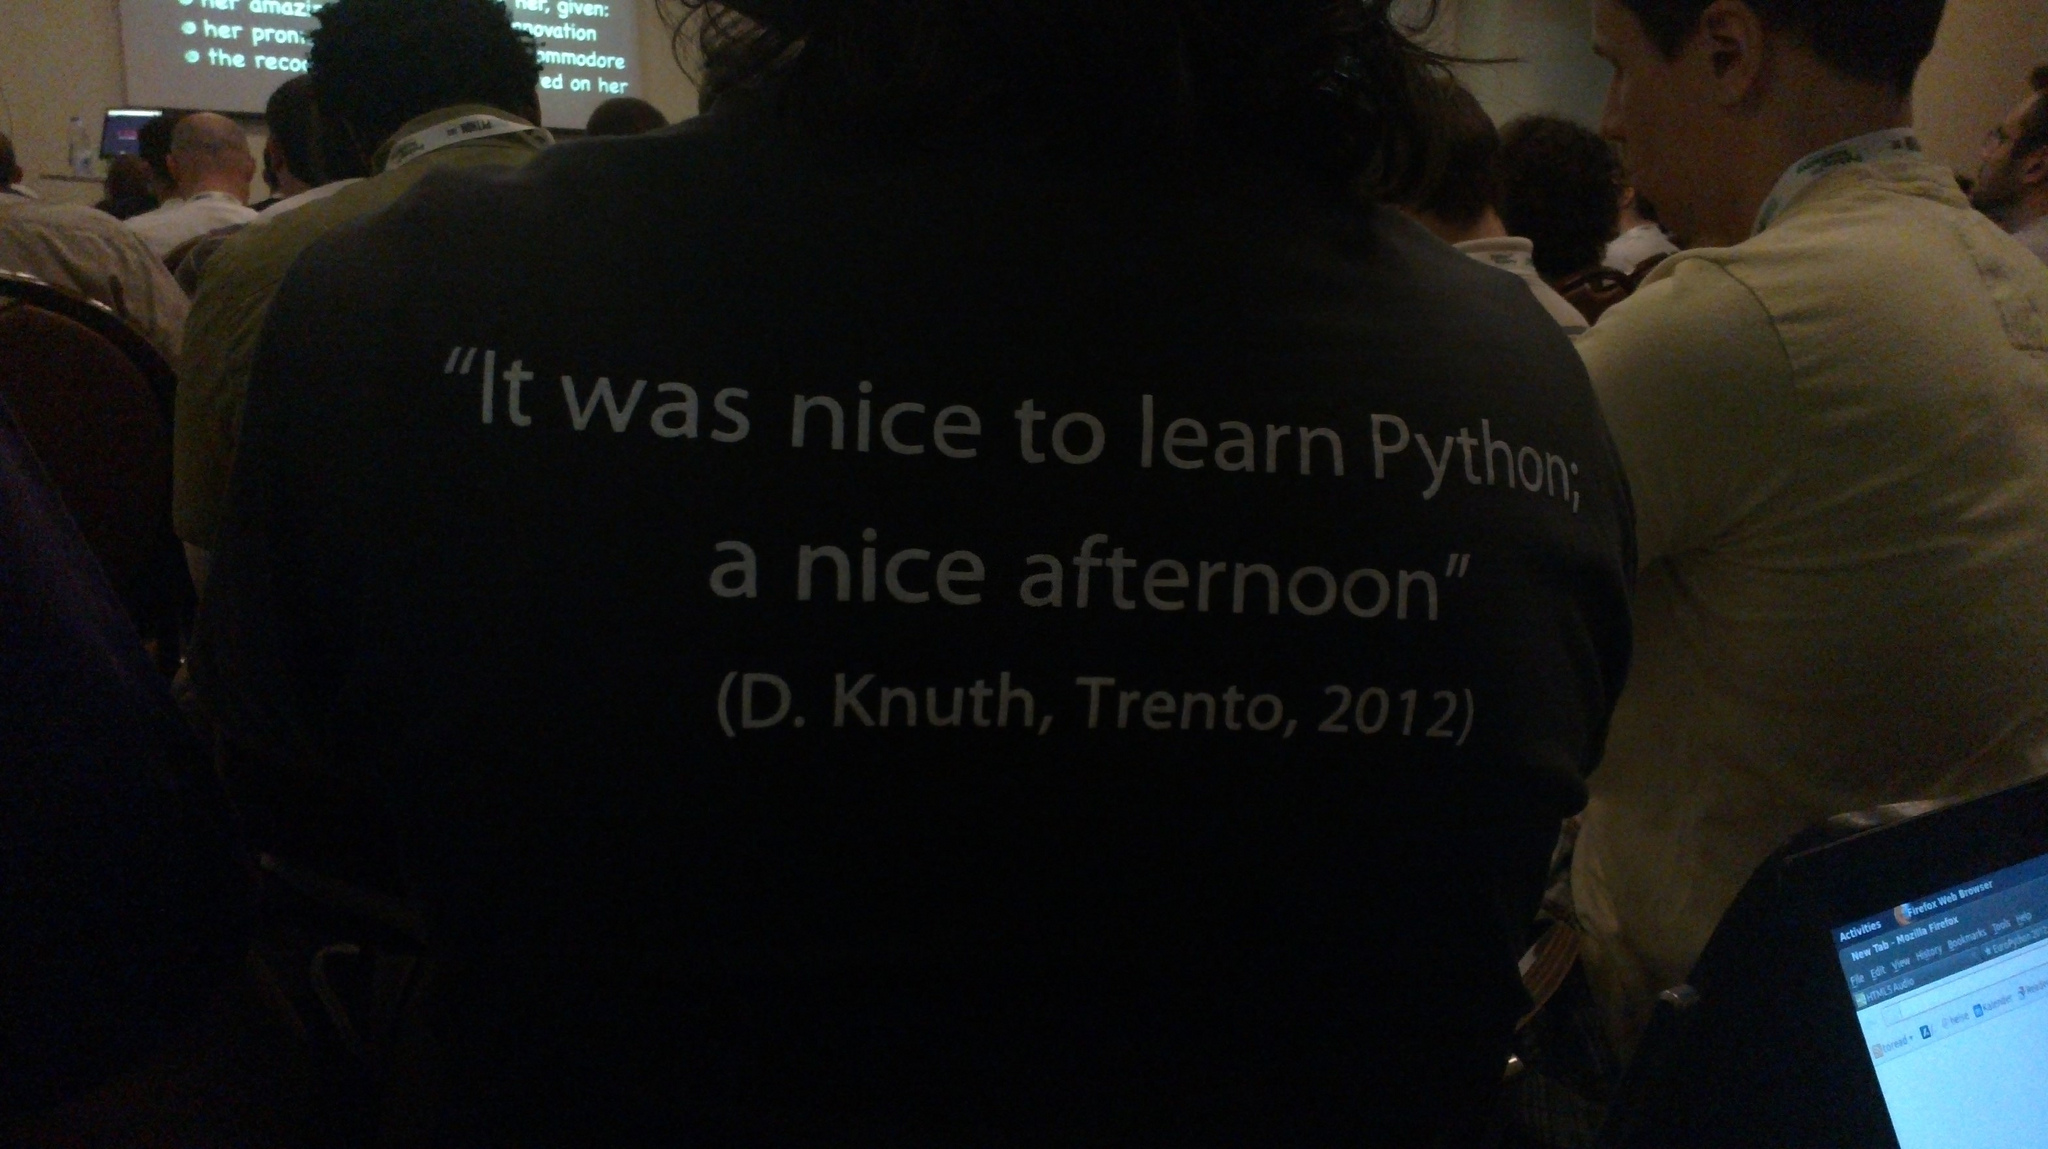
\includegraphics[scale=.2]{funnypython.jpg}
 \caption{Camisola cómica, realçando a facilidade de aprendizagem de Python. Fonte: Tumblr, thp4}
 \label{funnypython}
\end{figure}
\medskip

\subsubsection{Facilidade de uso}
Python tem uma grande vantagem no aspeto da facilidade de uso em relação ao Java pois é uma linguagem de alto nível que utiliza a indentação como meio de dividir código em módulos, o que em Java só pode ser feito através de chavetas. Para além de guiar melhor a leitura para um desenvolvedor, é também mais rápido de escrever. O uso de variáveis dinâmicas e de uma linguagem não tão rígida a nível de sintaxe também facilita muito a escrita em Python e a iniciação à programação, se esse for o caso. (\autoref{funnypython}). Por estas razões, programas em Python são mais rápidos de escrever e mais pequenos, em teoria (são tipicamente três a cinco vezes mais pequenos do que quando são escritos em Java \cite{officialpython}).
\medskip

\subsubsection{Estatísticas de uso global}
De acordo com Tiobe (\url{http://www.tiobe.com/}), em Fevereiro de 2015, a linguagem mais popular mundialmente é o C, seguido de perto por Java, com ratings de 16.488\% e 15.343\% (respetivamente). Python está em oitavo lugar, com um rating de 2.888\%, o que pode parecer uma diferença significativa (\cite{Tiobe}). Na realidade, Python tem crescido significativamente nos últimos anos, mas os avanços dos mais recentes softwares de \textit{smartphones} e \textit{tablets} (principalmente o sistema \textit{Android}) têm inflacionado bastante o uso de Java nos últimos anos.
Pelo referido no subcapítulo anterior, Python é uma das linguagens mais usadas para iniciação à programação. Um estudo (\url{http://cacm.acm.org/blogs/blog-cacm/176450-python-is-now-the-most-popular-introductory-teaching-language-at-top-us-universities/fulltext}) realizado nas universidades americanas mostra que é a linguagem mais usada na aprendizagem de programação, com algum avanço sobre Java (\cite{Pythonlearning}).


\part{Conclusão}

\chapter{Conclusão}
Java e Python são duas linguagens com propósitos diferentes, como foi possível constatar ao longo deste relatório. Python é uma linguagem mais simples, mais fácil de aprender e também mais rápida para desenvolvimento de projetos. É uma linguagem de scripting, pronta para correr em websites e servidores de maneira rápida e fácil. No entanto, a sua velocidade de execução é menor do que a de Java, devido ao facto de ser uma linguagem de maior abstração (o que envolve uma análise mais demorada das suas funções, métodos, objetos). Java tem a vantagem de ser uma linguagem mais robusta e segura, e ser atualmente uma das mais usadas mundialmente, principalmente em relação a fazer aplicações \textit{client-server} e aplicações para o sistema \textit{Android} (mobile), as quais têm uma grande importância na tecnologia atual. É, também, possível integrar as duas linguagens para fazer uma aplicação, usando Java como linguagem de nível médio e Python como "glue language", ou seja, uma linguagem que serve para integrar outras linguagens entre si.

Esperamos com este relatório ter explicitado as principais diferenças sintáticas das duas linguagens. Podíamos ter aprofundado mais em alguns capítulos, e até talvez fazer mais comparações sobre tópicos mais avançados, mas como ainda não nos sentimos confortáveis sobre esses temas, e como não tivemos muito tempo, preferimos ficar pelo básico e essencial.

\bibliography{pythonb}
\bibliographystyle{plain}

\end{document}
